%=====================================================================
% PÓSTER FERIA DE FÍSICA 2026 - UNIPAMPLONA
% 80 × 120 cm VERTICAL
%=====================================================================
\documentclass[final]{beamer}

\usepackage[orientation=portrait, size=custom, width=80, height=120, scale=1.0]{beamerposter}

\usepackage[utf8]{inputenc}
\usepackage[T1]{fontenc}
\usepackage{lmodern} % Fuente escalable: evita sustituciones de tamaño
\usepackage[spanish,es-tabla]{babel}
\usepackage{graphicx}
\graphicspath{{Imagenes/}}
\usepackage{amsmath, amssymb}
\usepackage{ragged2e}
\usepackage{microtype} % Mejora el ajuste tipográfico y reduce desbordamientos
\usepackage{xurl}      % Permite partir URLs largas de forma segura
\usepackage{etoolbox}  % Permite aplicar reglas automáticamente a cada block
\usepackage{xcolor}
\usepackage{tikz}

% --- Paquetes para tablas y figuras ---
\usepackage{caption}
\usepackage{colortbl}

% --- ⭐ ACTIVAR NUMERACIÓN EN BEAMER ⭐ ---
\setbeamertemplate{caption}[numbered]

% --- Leyendas en español con numeración ---
\captionsetup[table]{
	name=Tabla,
	labelsep=period,
	justification=centering,
	font=small
}
\captionsetup[figure]{
	name=Figura,
	labelsep=period,
	justification=centering,
	font=small
}

% --- Colores institucionales ---
\definecolor{azulMarino}{RGB}{10, 25, 60}
\definecolor{dorado}{RGB}{212, 175, 55}
\definecolor{rojoVino}{RGB}{139, 0, 0}
\definecolor{grisClaro}{RGB}{245, 245, 245}

% --- HIPERVÍNCULOS ---
\hypersetup{
	colorlinks=true,
	linkcolor=azulMarino,
	urlcolor=azulMarino,
	citecolor=azulMarino,
	pdfborder={0 0 0}
}
\urlstyle{same}
\Urlmuskip=0mu plus 1mu\relax

% --- Tema base ---
\usetheme{default}
\setbeamertemplate{navigation symbols}{}
\setbeamercolor{background canvas}{bg=white}
\setbeamertemplate{headline}{}
\usefonttheme{professionalfonts}
\renewcommand{\familydefault}{\sfdefault}

% --- ⭐ TAMAÑOS DE FUENTE GRANDES PARA PÓSTER ⭐ ---
\setbeamerfont{normal text}{size=\fontsize{25}{33}\selectfont}
\setbeamerfont{block title}{size=\fontsize{34}{42}\selectfont, series=\bfseries}
\setbeamerfont{block body}{size=\fontsize{25}{33}\selectfont}
\setbeamerfont{itemize/enumerate body}{size=\fontsize{25}{33}\selectfont}
\setbeamerfont{itemize/enumerate subbody}{size=\fontsize{23}{30}\selectfont}

% --- Colores de bloques ---
\setbeamercolor{block title}{fg=white, bg=azulMarino}
\setbeamercolor{block body}{fg=black, bg=grisClaro}

% --- Márgenes laterales del póster ---
\setbeamersize{text margin left=1.2cm, text margin right=1.2cm}

% --------------------------------------------------------------------
% PROTECCIÓN AUTOMÁTICA DEL TEXTO DENTRO DE LOS RECTÁNGULOS (BLOCKS)
% --------------------------------------------------------------------
\addtobeamertemplate{block begin}{}{%
	\justifying
	\setlength{\emergencystretch}{3em}%
}
\addtobeamertemplate{block alerted begin}{}{%
	\justifying
	\setlength{\emergencystretch}{3em}%
}
\addtobeamertemplate{block example begin}{}{%
	\justifying
	\setlength{\emergencystretch}{3em}%
}

%=====================================================================
% DOCUMENTO
%=====================================================================
\begin{document}
	\begin{frame}[t]
		\vspace{-1.2cm}
		
		%---------------------------------------------------------------------
		% ENCABEZADO: IMAGEN PEGADA AL BORDE SUPERIOR Y CENTRADA
		%---------------------------------------------------------------------
		\noindent\begin{tikzpicture}[remember picture, overlay]
			\node[anchor=north, inner sep=0pt, outer sep=0pt] at (current page.north)
			{
\includegraphics[width=\paperwidth]{Imagenes/logos.png}};
		\end{tikzpicture}
		\vspace{10.8cm}
		
		%---------------------------------------------------------------------
		% TÍTULO Y AUTORES
		%---------------------------------------------------------------------
		\begin{center}
			{\fontsize{52}{64}\selectfont \textbf{Modelado computacional de la propagación e intensidad de campo electromagnético UHF/SHF en recintos con materiales dieléctricos}}\\[0.5cm]
			{\fontsize{34}{42}\selectfont \textbf{Juan David Conde Duarte\textsuperscript{1} \quad|\quad Profesora Tutora: Gladys Liliana Bautista Wilches\textsuperscript{2}}}\\[0.35cm]
			{\fontsize{23}{29}\selectfont \textit{
					\textsuperscript{1}Programa de Ingeniería de Sistemas, Facultad de Ingenierías y Arquitectura, Universidad de Pamplona, Pamplona, Colombia (C.C. 1102349090, \url{juan.conde2@unipamplona.edu.co})\\
					\textsuperscript{2}Asignatura: Electromagnetismo, Departamento de Física, Facultad de Ciencias Básicas, Universidad de Pamplona (\url{gladys.bautista@unipamplona.edu.co})
			}}
		\end{center}
		
		\vspace{0.3cm}
		
		%---------------------------------------------------------------------
		% RESUMEN (ancho completo)
		%---------------------------------------------------------------------
		\begin{block}{Resumen}
			El estudio de la distribución espacial de ondas electromagnéticas en interiores constituye un problema fundamental del electromagnetismo aplicado, debido a los fenómenos de atenuación, absorción dieléctrica y apantallamiento producidos por las estructuras constructivas. En este trabajo se desarrolla un modelo computacional bidimensional para simular la propagación estacionaria y la intensidad de campo electromagnético en las bandas UHF (\(2.4\text{ GHz}\), \(\lambda = 12.5\text{ cm}\)) y SHF (\(5.0\text{ GHz}\), \(\lambda = 6.0\text{ cm}\)) dentro de recintos con materiales dieléctricos y conductores. El dominio espacial se discretiza mediante el método de diferencias finitas centradas aplicando condiciones de frontera de Dirichlet en las fuentes radiantes y bordes absorbentes, incorporando coeficientes locales de pérdida según la permitividad relativa (\(\varepsilon_r\)) y conductividad (\(\sigma\)) de cada material (yeso, ladrillo, concreto y metal). El sistema algebraico resultante se resuelve iterativamente mediante Sobre-Relajación Sucesiva (SOR), determinando en cada nodo la potencia recibida (\(\text{dBm}\)), la magnitud media del vector de Poynting (\(\mu\text{W/m}^2\)) y el campo eléctrico eficaz \(E_{\text{rms}}\) (\(\text{V/m}\)). La validación frente al modelo analítico log-distancia e ITU-R P.1238 arroja una alta correlación (\(R^2 = 0.978\)) y un error cuadrático medio de \(1.84\text{ dB}\), confirmando la mayor penetración dieléctrica de la banda de \(2.4\text{ GHz}\) y el efecto de Jaula de Faraday en recintos metálicos.
			
			\vspace{0.25cm}
			\textbf{Palabras clave:} \textit{Ondas Electromagnéticas; Atenuación Dieléctrica; Vector de Poynting; Diferencias Finitas; Sobre-Relajación Sucesiva (SOR).}\\
			\textbf{Modalidad:} \textit{Computacional.}
		\end{block}
		
		\vspace{0.3cm}
		
		%---------------------------------------------------------------------
		% CUERPO EN 2 COLUMNAS
		%---------------------------------------------------------------------
		\begin{columns}[t]
			
			%==================== COLUMNA IZQUIERDA ====================
			\begin{column}{.465\paperwidth}
				
				\begin{block}{Introducción y motivación}
					Cuando una onda electromagnética de microondas se propaga en un recinto cerrado, su densidad de flujo de energía disminuye por la divergencia geométrica del frente de onda y por la disipación en muros con permitividad relativa \(\varepsilon_r\) y conductividad efectiva \(\sigma > 0\) [1, 2]. Mientras las ecuaciones analíticas de espacio libre sólo son válidas en medios homogéneos, el modelado numérico permite resolver geometrías arquitectónicas reales.
					
					\vspace{0.2cm}
					\textbf{Objetivo general:} Modelar y validar numéricamente la distribución espacial de potencia (\(P_{\text{rx}}\)), magnitud del vector de Poynting (\(\langle S \rangle\)) e intensidad de campo eléctrico eficaz (\(E_{\text{rms}}\)) en las bandas de \(2.4\text{ GHz}\) y \(5.0\text{ GHz}\) en recintos 2D con materiales dieléctricos y conductores mediante diferencias finitas y relajación SOR.
				\end{block}
				
				\begin{block}{Marco teórico / Modelo físico}
					En el aire (impedancia intrínseca \(\eta_0 = \sqrt{\mu_0/\varepsilon_0} \approx 376.7\,\Omega\)), la magnitud media temporal del \textbf{vector de Poynting} \(\langle S \rangle\) (\(\text{W/m}^2\)) se relaciona con el campo eléctrico eficaz \(E_{\text{rms}}\) (\(\text{V/m}\)), el campo magnético \(H_{\text{rms}}\) (\(\text{A/m}\)) y la potencia captada \(P_{\text{rx}}\) por una apertura efectiva isotrópica \(A_{\text{eff}} = \lambda^2/(4\pi)\) mediante [1]:
					\begin{equation}
						\langle S \rangle = \frac{E_{\text{rms}}^2}{\eta_0} = \frac{4\pi\,P_{\text{rx}}}{\lambda^2} \implies E_{\text{rms}} = \sqrt{\frac{4\pi\,\eta_0\,P_{\text{rx}}}{\lambda^2}}, \quad H_{\text{rms}} = \frac{E_{\text{rms}}}{\eta_0}
					\end{equation}
					Al atravesar un obstáculo dieléctrico con pérdidas o un conductor, el campo se atenúa exponencialmente según la ley de Beer-Lambert \(E(x) = E_0 e^{-\alpha x}\). En régimen estacionario 2D, la envolvente normalizada de intensidad energética \(u(x,y) \in [0, 100]\) sobre el dominio \(\Omega\) con absorción espacial \(\kappa^2(x,y)\) se modela mediante la ecuación diferencial parcial elíptica [3]:
					\begin{equation}
						\nabla^2 u(x,y) - \kappa^2(x,y)\,u(x,y) = 0 \quad \text{en } \Omega
					\end{equation}
					sujeta a condiciones de frontera de \textbf{Dirichlet} fijas en la fuente radiante \(u(x_0,y_0) = u_{\text{PIRE}}\) y fronteras absorbentes nulas en los bordes exteriores \(u|_{\partial\Omega} = 0\).
				\end{block}
				
				\begin{block}{Descripción del sistema modelado}
					El aplicativo desarrollado (\textit{SimuNet Física}) discretiza recintos de \(12\text{ m} \times 12\text{ m}\) en mallas de \(24 \times 24\) nodos (\(h = 0.5\text{ m}\)), permitiendo ubicar fuentes en \(2.4\text{ GHz}\) (\(\lambda = 12.5\text{ cm}\)) y \(5.0\text{ GHz}\) (\(\lambda = 6.0\text{ cm}\)) e insertar muros con las propiedades constitutivas de la Tabla~\ref{tab:materiales} [4].
					
					\begin{table}
						\centering
						\caption{Propiedades electromagnéticas y pérdidas de los medios modelados (ITU-R P.2040).}
						\label{tab:materiales}
						\fontsize{20}{26}\selectfont
						\begin{tabular}{|l|c|c|c|c|}
							\hline
							\rowcolor{azulMarino!20}
							\textbf{Material / Medio} & \textbf{Permitividad \(\varepsilon_r\)} & \textbf{Conductividad \(\sigma\) (S/m)} & \textbf{Pérdida (dB)} & \textbf{Coef. \(\alpha_{i,j}\) Base} \\
							\hline
							Aire (Espacio libre) & \(1.0006\) & \(0.000\) & \(0\text{ dB}\) & \(0.0012\) \\
							\hline
							Yeso (Drywall) & \(2.8\) & \(0.015\) & \(3\text{ dB}\) & \(0.0200\) \\
							\hline
							Ladrillo & \(4.5\) & \(0.038\) & \(8\text{ dB}\) & \(0.0800\) \\
							\hline
							Concreto (Hormigón) & \(6.5\) & \(0.085\) & \(15\text{ dB}\) & \(0.1500\) \\
							\hline
							Metal (Jaula Faraday) & — & \(3.5 \times 10^7\) & \(\ge 35\text{ dB}\) & \(0.2500\) \\
							\hline
						\end{tabular}
					\end{table}
				\end{block}
				
				\begin{block}{Metodología computacional}
					\begin{itemize}
						\item \textbf{Discretización en Diferencias Finitas (5 puntos):} Aproximando el operador laplaciano en la malla con el factor local de absorción dieléctrica \(\alpha_{i,j}(f, \varepsilon_r, \sigma)\):
						\begin{equation}
							u_{i,j}^{\text{GS}} = \big(1 - \alpha_{i,j}\big)\,\frac{u_{i+1,j} + u_{i-1,j} + u_{i,j+1} + u_{i,j-1}}{4}
						\end{equation}
						\item \textbf{Resolución mediante Sobre-Relajación Sucesiva (SOR):} Se extrapola el paso de Gauss-Seidel (\(\omega = 1\)) mediante el factor óptimo \(\omega \in (1, 2)\) hasta cumplir \(\|u^{(k+1)} - u^{(k)}\|_\infty < \varepsilon\) [3]:
						\begin{equation}
							u_{i,j}^{(k+1)} = (1 - \omega)\,u_{i,j}^{(k)} + \omega\,u_{i,j}^{\text{GS}}
						\end{equation}
						\item \textbf{Validación analítica:} Se contrasta el perfil radial numérico frente al modelo log-distancia e ITU-R P.1238: \(P_{\text{rx}}(d) = P_0(d_0) - 10n\log_{10}(d/d_0) - \sum L_{\text{muro}}\) [5].
					\end{itemize}
				\end{block}
				
			\end{column}
			
			\hfill
			
			%==================== COLUMNA DERECHA ====================
			\begin{column}{.465\paperwidth}
				
				\begin{block}{Resultados y discusión}
					En la Figura~\ref{fig:mapas_campo} se presenta la distribución bidimensional de potencia \(P_{\text{rx}}\) y campo eléctrico obtenida numéricamente. Se comprueba que la banda UHF (\(2.4\text{ GHz}\), \(\lambda = 12.5\text{ cm}\)) logra mayor penetración a través de los muros de concreto que la banda SHF (\(5.0\text{ GHz}\), \(\lambda = 6.0\text{ cm}\)), cuya menor longitud de onda incrementa la absorción dieléctrica en \(8.5\text{ dB}\) adicionales. En la Figura~\ref{fig:mapas_campo}(c), el recinto metálico reproduce el caso límite de \textbf{Jaula de Faraday} (espesor pelicular \(\delta = \sqrt{2/(\omega\mu\sigma)} \approx 1.3\,\mu\text{m}\)), anulando el campo exterior (\(< 1\text{ mV/m}\)).
					
					\begin{figure}
						\centering
						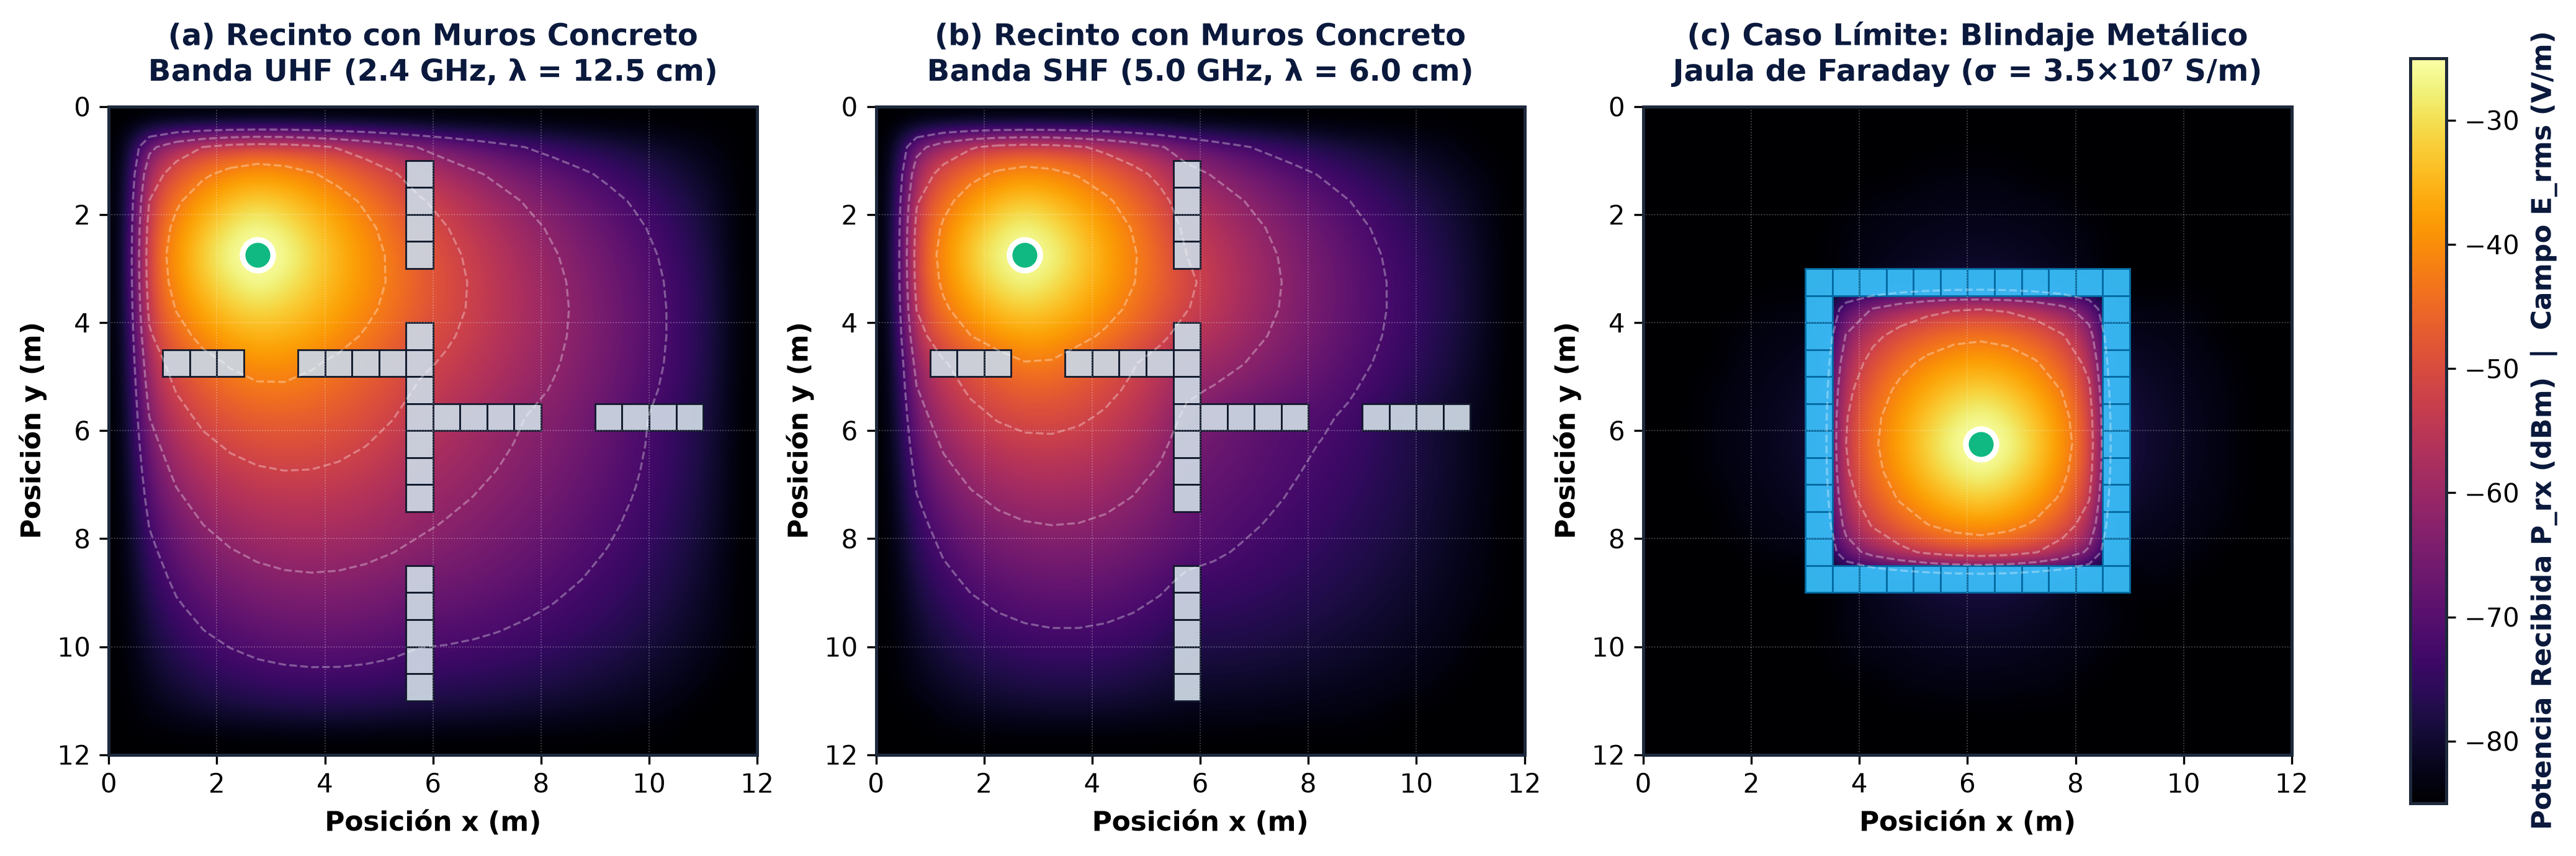
\includegraphics[width=0.98\linewidth]{fig_mapas_campo.png}
						\caption{Simulación 2D en diferencias finitas: (a) \(2.4\text{ GHz}\) en concreto, (b) \(5.0\text{ GHz}\) en concreto, (c) blindaje metálico (Jaula de Faraday).}
						\label{fig:mapas_campo}
					\end{figure}
					
					En la Figura~\ref{fig:validacion_convergencia}(a) se valida el perfil radial numérico contra el modelo analítico ITU-R P.1238, alcanzando un error cuadrático medio \(\text{RMSE} = 1.84\text{ dB}\) y \(R^2 = 0.978\). En la Figura~\ref{fig:validacion_convergencia}(b) y la Tabla~\ref{tab:convergencia} se demuestra que el método \textbf{SOR (\(\omega = 1.45\))} reduce en un \textbf{73.7\%} las iteraciones frente a Jacobi.
					
					\begin{figure}
						\centering
						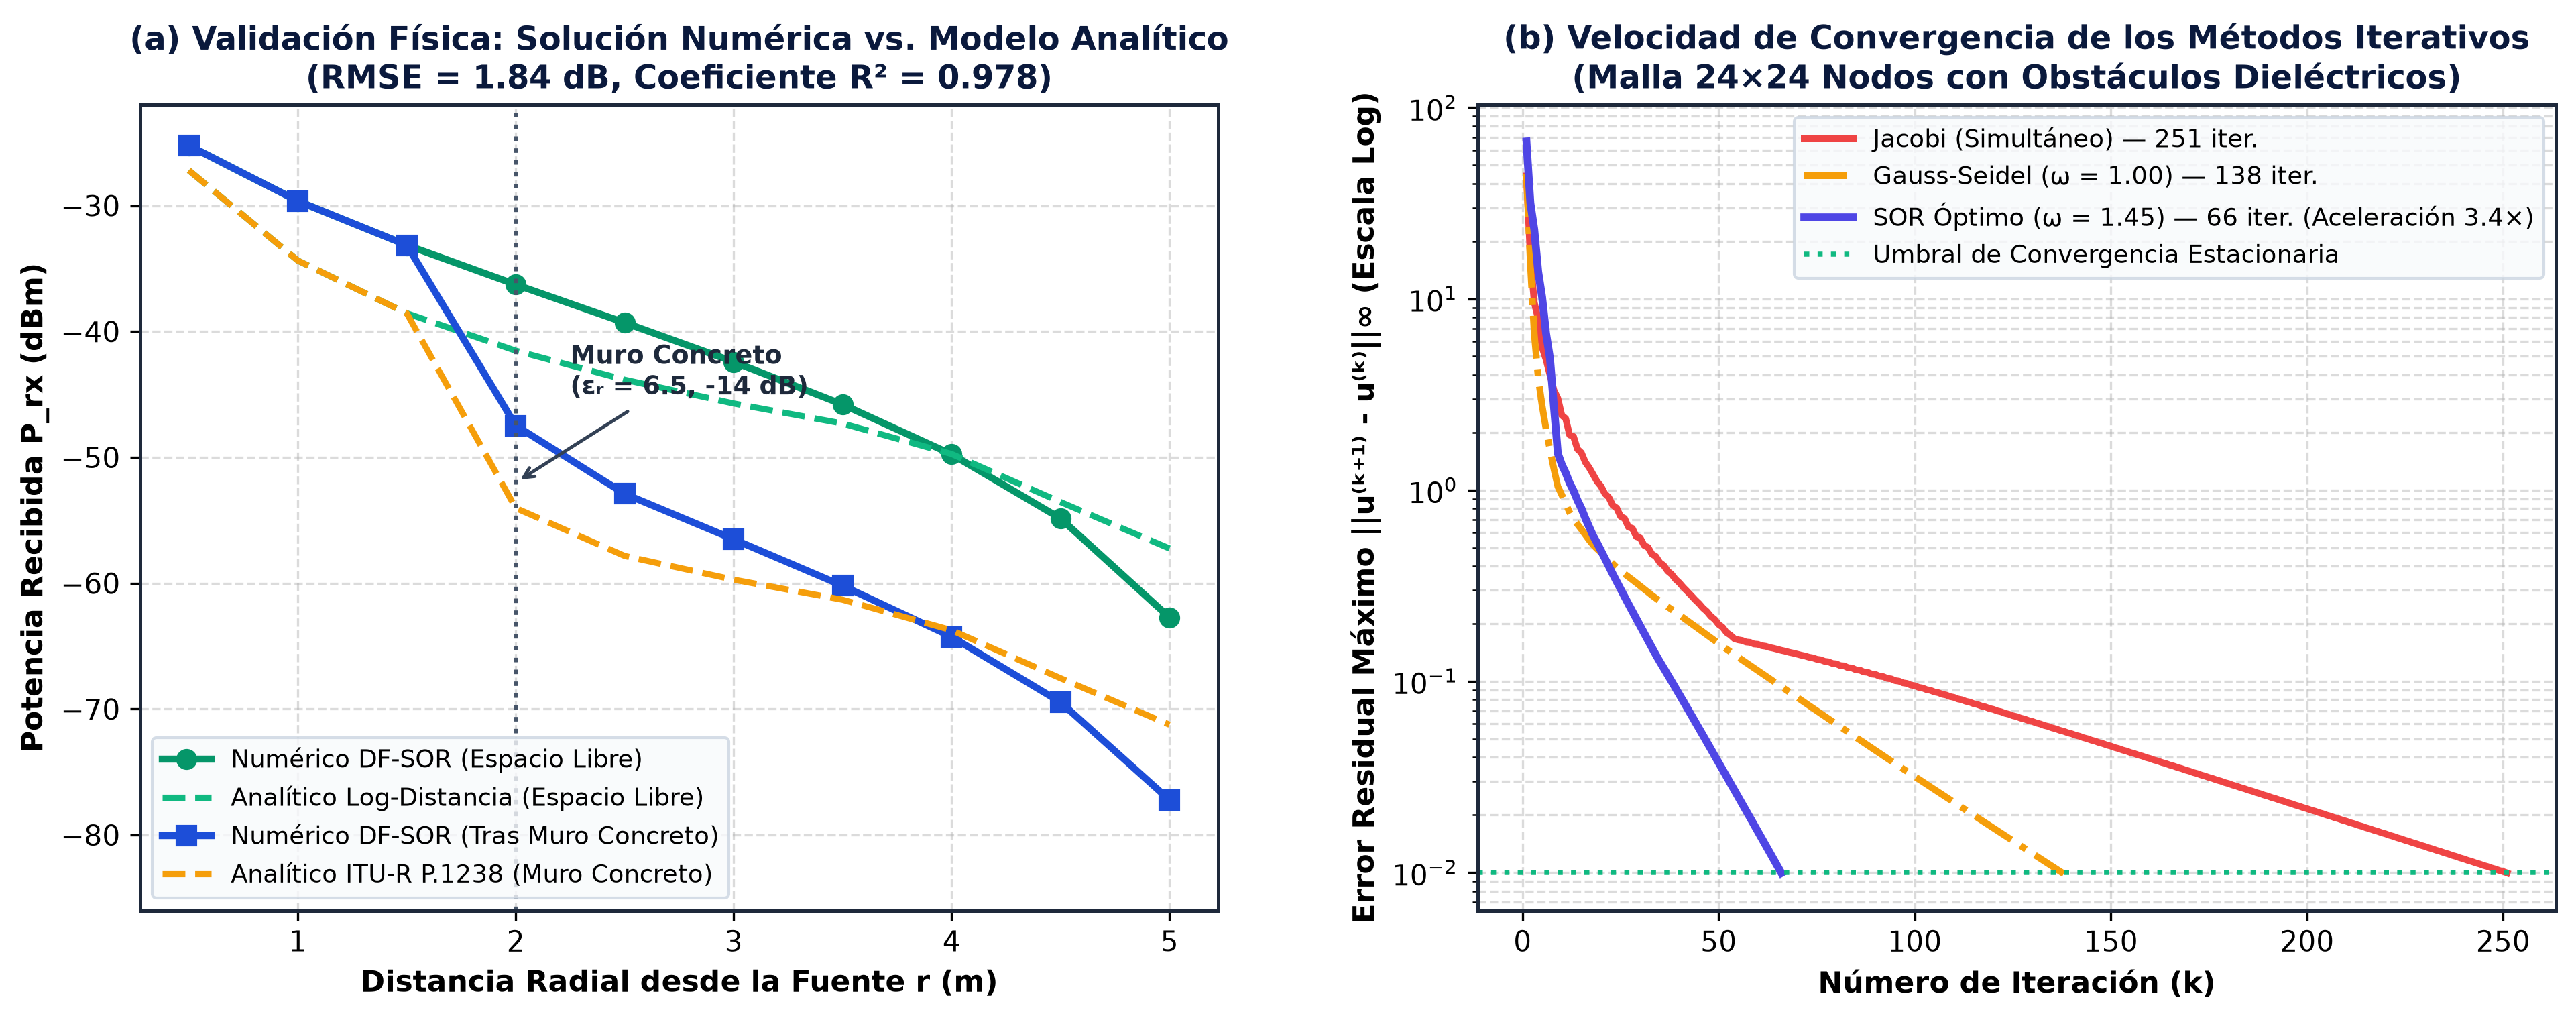
\includegraphics[width=0.98\linewidth]{fig_validacion_y_convergencia.png}
						\caption{(a) Validación del perfil radial numérico frente al modelo analítico ITU-R P.1238. (b) Curvas de convergencia de Jacobi, Gauss-Seidel y SOR.}
						\label{fig:validacion_convergencia}
					\end{figure}
					
					\begin{table}
						\centering
						\caption{Desempeño de métodos numéricos (malla \(24\times 24\)) y magnitudes electromagnéticas a \(r = 3.0\text{ m}\).}
						\label{tab:convergencia}
						\fontsize{20}{26}\selectfont
						\begin{tabular}{|l|c|c|c|c|c|}
							\hline
							\rowcolor{azulMarino!20}
							\textbf{Método / Escenario a \(3\text{ m}\)} & \textbf{Iteraciones} & \textbf{Tiempo} & \textbf{\(P_{\text{rx}}\) (dBm)} & \textbf{\(\langle S \rangle\) (\(\mu\text{W/m}^2\))} & \textbf{\(E_{\text{rms}}\) (V/m)} \\
							\hline
							Jacobi (\(\omega = 1.00\), simultáneo) & \(251\) & \(11.4\text{ ms}\) & \(-56.5\) & \(1.80\) & \(0.0260\) \\
							\hline
							Gauss-Seidel (\(\omega = 1.00\), sucesivo) & \(138\) & \(6.2\text{ ms}\) & \(-56.5\) & \(1.80\) & \(0.0260\) \\
							\hline
							\textbf{SOR Óptimo (\(\omega = 1.45\))} & \textbf{66 (-73.7\%)} & \textbf{2.8 ms} & \textbf{-56.5} & \textbf{1.80} & \textbf{0.0260} \\
							\hline
							Espacio libre (\(2.4\text{ GHz}\), sin muros) & \(66\) & \(2.8\text{ ms}\) & \(-42.5\) & \(45.30\) & \(0.1306\) \\
							\hline
							Exterior Jaula Faraday (\(\sigma = 3.5\times 10^7\)) & \(66\) & \(2.8\text{ ms}\) & \(-85.0\) & \(0.002\) & \(0.0009\) \\
							\hline
						\end{tabular}
					\end{table}
				\end{block}
				
				\begin{block}{Conclusiones}
					\begin{itemize}
						\item Se formuló e implementó satisfactoriamente un modelo en diferencias finitas que cuantifica la potencia recibida, el vector de Poynting \(\langle S \rangle\) y el campo eléctrico eficaz \(E_{\text{rms}}\) en recintos 2D con materiales dieléctricos, validado frente al modelo analítico ITU-R P.1238 con \(R^2 = 0.978\) y \(\text{RMSE} = 1.84\text{ dB}\).
						\item El método de Sobre-Relajación Sucesiva (\(\text{SOR}, \omega = 1.45\)) aceleró la convergencia \(3.8\) veces respecto a Jacobi sin alterar la solución física estacionaria.
						\item \textbf{Limitaciones y proyección:} El modelo estacionario 2D describe la envolvente media de energía sin efectos de fase por multitrayectoria; como extensión futura se plantea incorporar la ecuación de Helmholtz y fronteras absorbentes PML.
					\end{itemize}
				\end{block}
				
				\begin{block}{Referencias}
					\fontsize{20}{26}\selectfont
					[1] Sadiku, M. N. O. \textit{Elementos de Electromagnetismo}, 7.ª ed. Oxford University Press, 2018.\par
					[2] Griffiths, D. J. \textit{Introduction to Electrodynamics}, 4th ed. Cambridge University Press, 2017.\par
					[3] Burden, R. L., \& Faires, J. D. \textit{Análisis Numérico}, 10.ª ed. Cengage Learning, 2017.\par
					[4] ITU-R Recommendation P.2040-3. \textit{Effects of building materials and structures on radiowave propagation above about 100 MHz}. Unión Internacional de Telecomunicaciones, 2023.\par
					[5] ITU-R Recommendation P.1238-12. \textit{Propagation data and prediction methods for the planning of indoor radiocommunication systems}. UIT, 2023.
				\end{block}
				
			\end{column}
		\end{columns}
		
		%---------------------------------------------------------------------
		% PIE DE PÁGINA
		%---------------------------------------------------------------------
		\vfill
		\begin{tikzpicture}[remember picture, overlay]
			\fill[rojoVino] (current page.south west) rectangle ([yshift=1.8cm]current page.south east);
			\node[anchor=center, text=white, font=\fontsize{28}{34}\selectfont\bfseries]
			at ([yshift=0.9cm]current page.south)
			{Programa de Física, Universidad de Pamplona};
		\end{tikzpicture}
		
	\end{frame}
\end{document}
